%%%%%%%%%%%%%%%%%%%%% chapter.tex %%%%%%%%%%%%%%%%%%%%%%%%%%%%%%%%%
%
% sample chapter
%
% Use this file as a template for your own input.
%
%%%%%%%%%%%%%%%%%%%%%%%% Springer-Verlag %%%%%%%%%%%%%%%%%%%%%%%%%%
%\motto{Use the template \emph{chapter.tex} to style the various elements of your chapter content.}


\chapter{Ninety-Nine Lisp Problems}
\label{cha:ninety-nine-lisp-problems}

\section*{Working with lists}
\label{sec:99-problems-}

\subsection*{{P01} (*) Find the last box of a list.}
\label{sec:99-problems-P01}

\begin{wideverbatim}

(de my-last (Lst)
   (tail 1 Lst) )

\end{wideverbatim}

\begin{wideverbatim}
   : (my-last '(a b c d))
   -> (d)
\end{wideverbatim}

\subsection*{{P02} (*) Find the last but one box of a
list.}
\label{sec:99-problems-P02}

\begin{wideverbatim}

(de my-but-last (Lst)
   (tail 2 Lst) )

\end{wideverbatim}

\begin{wideverbatim}
   : (my-but-last '(a b c d))
   -> (c d)
\end{wideverbatim}

\subsection*{{P03} (*) Find the K'th element of a list.}
\label{sec:99-problems-P03}

The first element in the list is number 1.

\begin{wideverbatim}

(de element-at (Lst N)
   (get Lst N) )

\end{wideverbatim}

\begin{wideverbatim}
   : (element-at '(a b c d e) 3)
   -> c
\end{wideverbatim}

\subsection*{{P04} (*) Find the number of elements of a
list.}
\label{sec:99-problems-P04}

\begin{wideverbatim}

(def 'comprimento length)

\end{wideverbatim}

\subsection*{{P05} (*) Reverse a list.}
\label{sec:99-problems-P05}

\begin{wideverbatim}

(def 'inverte reverse)

\end{wideverbatim}

\subsection*{{P06} (*) Find out whether a list is a
palindrome.}
\label{sec:99-problems-P06}

A palindrome can be read forward or backward; e.g. (x a m a x).

\begin{wideverbatim}

(de palin (Lst)
   (= Lst (reverse Lst)) )

\end{wideverbatim}

\subsection*{{P07} (**) Flatten a nested list
structure.}
\label{sec:99-problems-P07}

Transform a list, possibly holding lists as elements into a `flat' list
by replacing each list with its elements (recursively).

\begin{wideverbatim}

(de flatten (Lst)
   (fish atom Lst) )

\end{wideverbatim}

\begin{wideverbatim}
   : (my-flatten '(a (b (c d) e)))
   -> (a b c d e)
\end{wideverbatim}


\subsection*{{P08} (**) Eliminate consecutive duplicates
of list elements.}
\label{sec:99-problems-P08}

If a list contains repeated elements they should be replaced with a
single copy of the element. The order of the elements should not be
changed.

\begin{wideverbatim}

(de compress (Lst)
   (mapcon
      '((L)
         (unless (= (car L) (cadr L))
            (cons (car L)) ) )
      Lst ) )

\end{wideverbatim}

\begin{wideverbatim}
   : (compress '(a a a a b c c a a d e e e e))
   -> (a b c a d e)
\end{wideverbatim}


\pagebreak{}
\subsection*{{P09} (**) Pack consecutive duplicates of
list elements into sublists.}
\label{sec:99-problems-P09}

If a list contains repeated elements they should be placed in separate
sublists.

\begin{wideverbatim}

(de consecDups (Lst)
   (make
      (let Last NIL
         (for X Lst
            (if (= X (car Last))
               (conc Last (cons X))
               (link (setq Last (cons X))) ) ) ) ) )

\end{wideverbatim}

\begin{wideverbatim}
   : (consecDups '(a a a a b c c a a d e e e e))
   -> ((a a a a) (b) (c c) (a a) (d) (e e e e))
\end{wideverbatim}

\subsection*{{P10} (*) Run-length encoding of a list.}
\label{sec:99-problems-P10}

Use the result of problem P09 to implement the so-called run-length
encoding data compression method. Consecutive duplicates of elements are
encoded as lists (N E) where N is the number of duplicates of the
element E.

\begin{wideverbatim}

(load "p09.l")

(de encode (Lst)
   (mapcar
      '((X) (list (length X) (car X)))
      (consecDups Lst) ) )

\end{wideverbatim}

\begin{wideverbatim}
   : (encode '(a a a a b c c a a d e e e e))
   -> ((4 a) (1 b) (2 c) (2 a) (1 d)(4 e))
\end{wideverbatim}

\pagebreak{}
\subsection*{{P11} (*) Modified run-length encoding.}
\label{sec:99-problems-P11}

Modify the result of problem P10 in such a way that if an element has no
duplicates it is simply copied into the result list. Only elements with
duplicates are transferred as (N E) lists.

\begin{wideverbatim}

(load "p09.l")

(de encode-modified (Lst)
   (mapcar
      '((X)
         (if (cdr X)
            (list (length X) (car X))
            (car X) ) )
      (consecDups Lst) ) )

\end{wideverbatim}

\begin{wideverbatim}
   : (encode-modified '(a a a a b c c a a d e e e e))
   -> ((4 a) b (2 c) (2 a) d (4 e))
\end{wideverbatim}

\subsection*{{P12} (**) Decode a run-length encoded
list.}
\label{sec:99-problems-P12}

Given a run-length code list generated as specified in problem P11.
Construct its uncompressed version.

\begin{wideverbatim}

(de decode (Lst)
   (make
      (for X Lst
         (if (atom X)
            (link X)
            (do (car X) (link (cadr X))) ) ) ) )

\end{wideverbatim}

\begin{wideverbatim}
   : (decode '((4 a) b (2 c) (2 a) d (4 e)))
   -> (a a a a b c c a a d e e e e)
\end{wideverbatim}

\pagebreak{}
\subsection*{{P13} (**) Run-length encoding of a list
(direct solution).}
\label{sec:99-problems-P13}

Implement the so-called run-length encoding data compression method
directly. I.e. don't explicitly create the sublists containing the
duplicates, as in problem P09, but only count them. As in problem P11,
simplify the result list by replacing the singleton lists (1 X) by X.

\begin{wideverbatim}

(de encode-direct (Lst)
   (make
      (while Lst
         (let (N 1  X)
            (while (= (setq X (pop 'Lst)) (car Lst))
               (inc 'N) )
            (link (if (= 1 N) X (list N X))) ) ) ) )

\end{wideverbatim}

\begin{wideverbatim}
   : (encode-direct '(a a a a b c c a a d e e e e))
   -> ((4 a) b (2 c) (2 a) d (4 e))
\end{wideverbatim}

\subsection*{{P14} (*) Duplicate the elements of a
list.}
\label{sec:99-problems-P14}

\begin{wideverbatim}

(de dupli (Lst)
   (mapcan list Lst Lst) )

\end{wideverbatim}

\begin{wideverbatim}
   : (dupli '(a b c c d))
   -> (a a b b c c c c d d)
\end{wideverbatim}

\pagebreak{}
\subsection*{{P15} (**) Replicate the elements of a list
a given number of times.}
\label{sec:99-problems-P15}

\begin{wideverbatim}

(de repli (Lst N)
   (mapcan '((X) (need N NIL X)) Lst) )

\end{wideverbatim}

\begin{wideverbatim}
   : (repli '(a b c) 3)
   -> (a a a b b b c c c)
\end{wideverbatim}


\subsection*{{P16} (**) Drop every N'th element from a
list.}
\label{sec:99-problems-P16}

\begin{wideverbatim}

(de drop (Lst N)
   (make
      (for (I . X) Lst
         (unless (=0 (% I N))
            (link X) ) ) ) )

\end{wideverbatim}

\begin{wideverbatim}
   : (drop '(a b c d e f g h i k) 3)
   -> (a b d e g h k)
\end{wideverbatim}


\subsection*{{P17} (*) Split a list into two parts; the
length of the first part is given.}
\label{sec:99-problems-P17}

Do not use any predefined predicates.

\begin{wideverbatim}

(de splitAt (Lst N)
   (list (cut N 'Lst) Lst) )

\end{wideverbatim}

\begin{wideverbatim}
   : (splitAt '(a b c d e f g h i k) 3)
   -> ((a b c) (d e f g h i k))
\end{wideverbatim}


\pagebreak{}
\subsection*{{P18} (**) Extract a slice from a list.}
\label{sec:99-problems-P18}

Given two indices, I and K, the slice is the list containing the
elements between the I'th and K'th element of the original list (both
limits included). Start counting the elements with 1.

\begin{wideverbatim}

(de slice (Lst I K)
   (head (inc (- K I)) (nth Lst I)) )

\end{wideverbatim}

\begin{wideverbatim}
   : (slice '(a b c d e f g h i k) 3 7)
   -> (c d e f g)
\end{wideverbatim}


\subsection*{{P19} (**) Rotate a list N places to the
left.}
\label{sec:99-problems-P19}

\begin{wideverbatim}

(de rotate (Lst N)
   (setq Lst (copy Lst))
   (do
      (if (lt0 N)
         (- N)
         (- (length Lst) N) )
      (rot Lst) ) )

\end{wideverbatim}

\begin{wideverbatim}
   : (rotate '(a b c d e f g h) 3)
   -> (d e f g h a b c)

   : (rotate '(a b c d e f g h) -2)
   -> (g h a b c d e f)
\end{wideverbatim}

Hint: Use the predefined functions length and append, as well as the
result of problem P17.


\pagebreak{}
\subsection*{{P20} (*) Remove the K'th element from a
list.}
\label{sec:99-problems-P20}

\begin{wideverbatim}

(de remove-at (Lst N)
   (remove N Lst) )

\end{wideverbatim}

\begin{wideverbatim}
   : (remove-at '(a b c d) 2)
   -> (a c d)
\end{wideverbatim}

\subsection*{{P21} (*) Insert an element at a given
position into a list.}
\label{sec:99-problems-P21}

\begin{wideverbatim}

(de insert-at (X Lst N)
   (insert N Lst X) )

\end{wideverbatim}

\begin{wideverbatim}
   : (insert-at 'alfa '(a b c d) 2)
   -> (a alfa b c d)
\end{wideverbatim}

\subsection*{{P22} (*) Create a list containing all
integers within a given range.}
\label{sec:99-problems-P22}

If first argument is smaller than second, produce a list in decreasing
order.

\begin{wideverbatim}

# 'range' is built-in
# A simplified implementation might be

(de my-range (A B)
   (let S (if (> B A) 1 -1)
      (make
         (until (= A B)
            (link A)
            (inc 'A S) ) ) ) )

\end{wideverbatim}

\begin{wideverbatim}
   : (range 4 9)
   -> (4 5 6 7 8 9)
\end{wideverbatim}


\pagebreak{}
\subsection*{{P23} (**) Extract a given number of
randomly selected elements from a list.}
\label{sec:99-problems-P23}

The selected items shall be returned in a list.

\begin{wideverbatim}

(de rnd-select (Lst N)
   (make
      (until (=0 N)
         (when (>= N (rand 1 (length Lst)))
            (link (car Lst))
            (dec 'N) )
         (pop 'Lst) ) ) )

\end{wideverbatim}

\begin{wideverbatim}
   : (rnd-select '(a b c d e f g h) 3)
   -> (e d a)
\end{wideverbatim}

Hint: Use the built-in random number generator and the result of problem
P20.

\subsection*{{P24} (*) Lotto: Draw N different random
numbers from the set 1..M.}
\label{sec:99-problems-P24}

The selected numbers shall be returned in a list.

\begin{wideverbatim}

(load "p23.l")

(de lotto-select (Cnt Max)
   (rnd-select (range 1 Max) Cnt) )

\end{wideverbatim}

\begin{wideverbatim}
   : (lotto-select 6 49)
   -> (23 1 17 33 21 37)
\end{wideverbatim}

Hint: Combine the solutions of problems P22 and P23.

\pagebreak{}
\subsection*{{P25} (*) Generate a random permutation of
the elements of a list.}
\label{sec:99-problems-P25}

\begin{wideverbatim}

(de rnd-permu (Lst)
   (by '(NIL (rand)) sort Lst) )

\end{wideverbatim}

\begin{wideverbatim}
   : (rnd-permu '(a b c d e f))
   -> (b a d c e f)
\end{wideverbatim}

Hint: Use the solution of problem P23.


\subsection*{{P26} (**) Generate the combinations of K
distinct objects chosen from the N elements of a list}
\label{sec:99-problems-P26}

In how many ways can a committee of 3 be chosen from a group of 12
people? We all know that there are C(12,3) = 220 possibilities (C(N,K)
denotes the well-known binomial coefficients). For pure mathematicians,
this result may be great. But \emph{we} want to really generate all the
possibilities in a list.

\begin{wideverbatim}

(de combination (N Lst)
   (cond
      ((=0 N) '(NIL))
      ((not Lst))
      (T
         (conc
            (mapcar
               '((X) (cons (car Lst) X))
               (combination (dec N) (cdr Lst)) )
            (combination N (cdr Lst)) ) ) ) )

\end{wideverbatim}

\begin{wideverbatim}
   : (combination 3 '(a b c d e f))
   -> ((a b c) (a b d) (a b e) ... )
\end{wideverbatim}

\pagebreak{}
\subsection*{{P27} (**) Group the elements of a set into
disjoint subsets.}
\label{sec:99-problems-P27}

a) In how many ways can a group of 9 people work in 3 disjoint subgroups
of 2, 3 and 4 persons? Write a function that generates all the
possibilities and returns them in a list.

\begin{wideverbatim}
   : (group3 '(aldo beat carla david evi flip gary hugo ida))
   -> (((aldo beat) (carla david evi) (flip gary hugo ida))
   ... )
\end{wideverbatim}

b) Generalize the above predicate in a way that we can specify a list of
group sizes and the predicate will return a list of groups.

\begin{wideverbatim}
   : (subsets '(aldo beat carla david evi flip gary hugo ida) '(2 2 5))
   -> (((aldo beat) (carla david) (evi flip gary hugo ida))
   ... )
\end{wideverbatim}

Note that we do not want permutations of the group members; i.e. ((aldo
beat) \ldots{}) is the same solution as ((beat aldo) \ldots{}). However,
we make a difference between ((aldo beat) (carla david) \ldots{}) and
((carla david) (aldo beat) \ldots{}).

You may find more about this combinatorial problem in a good book on
discrete mathematics under the term ``multinomial coefficients''.

\begin{wideverbatim}

(load "p26.l")

(de subsets (Set Lst)
   (if (cdr Lst)
      (mapcan
         '((C)
            (mapcar
               '((S) (cons C S))
               (subsets (diff Set C) (cdr Lst)) ) )
         (combination (car Lst) Set) )
      (cons (cons Set)) ) )

\end{wideverbatim}

\pagebreak{}
\subsection*{{P28} (**) Sorting a list of lists
according to length of sublists}
\label{sec:99-problems-P28}

a) We suppose that a list contains elements that are lists themselves.
The objective is to sort the elements of this list according to their
\textbf{length}. E.g. short lists first, longer lists later, or vice
versa.

\begin{wideverbatim}
   : (lsort '((a b c) (d e) (f g h) (d e) (i j k l) (m n) (o)))
   -> ((o) (d e) (d e) (m n) (a b c) (f g h) (i j k l))
\end{wideverbatim}

b) Again, we suppose that a list contains elements that are lists
themselves. But this time the objective is to sort the elements of this
list according to their \textbf{length frequency}; i.e., in the default,
where sorting is done ascendingly, lists with rare lengths are placed
first, others with a more frequent length come later.

\begin{wideverbatim}
   : (lfsort '((a b c) (d e) (f g h) (d e) (i j k l) (m n) (o)))
   -> ((i j k l) (o) (a b c) (f g h) (d e) (d e) (m n))
\end{wideverbatim}

Note that in the above example, the first two lists in the result have
length 4 and 1, both lengths appear just once. The third and forth list
have length 3 which appears twice (there are two list of this length).
And finally, the last three lists have length 2. This is the most
frequent length.

\begin{wideverbatim}

(de lsort (Lst)
   (by length sort Lst) )

(de lfsort (Lst)
   (by
      '((X)
         (cnt
            '((L) (= (length L) (length X)))
            Lst ) )
      sort Lst ) )

\end{wideverbatim}


\pagebreak{}
\section*{Arithmetic}

\subsection*{{P31} (**) Determine whether a given
integer number is prime.}
\label{sec:99-problems-P31}

\begin{wideverbatim}

(de is-prime (N)
   (or
      (= N 2)
      (and
         (> N 1)
         (bit? 1 N)
         (for (D 3  T  (+ D 2))
            (T (> D (sqrt N)) T)
            (T (=0 (% N D)) NIL) ) ) ) )

\end{wideverbatim}

\begin{wideverbatim}
   : (is-prime 7)
   -> T
\end{wideverbatim}

\subsection*{{P32} (**) Determine the greatest common
divisor of two positive integer numbers.}
\label{sec:99-problems-P32}

Use Euclid's algorithm.

\begin{wideverbatim}

(de gcd (A B)
   (until (=0 B)
      (let M (% A B)
         (setq A B B M) ) )
   (abs A) )

\end{wideverbatim}

\begin{wideverbatim}
   : (gcd 36 63)
   -> 9
\end{wideverbatim}

\pagebreak{}
\subsection*{{P33} (*) Determine whether two positive
integer numbers are coprime.}
\label{sec:99-problems-P33}

Two numbers are coprime if their greatest common divisor equals 1.

\begin{wideverbatim}

(load "p32.l")

(de coprime (A B)
   (= 1 (gcd A B)) )

\end{wideverbatim}

\begin{wideverbatim}
   : (coprime 35 64)
   -> T
\end{wideverbatim}


\subsection*{{P34} (**) Calculate Euler's totient
function phi(m).}
\label{sec:99-problems-P34}

Euler's so-called totient function phi(m) is defined as the number of
positive integers r (1 \&lt;= r \&lt; m) that are coprime to m.

Example: m = 10: r = 1,3,7,9; thus phi(m) = 4. Note the special case:
phi(1) = 1.

\begin{wideverbatim}
   : (totient-phi 10)
   -> 4
\end{wideverbatim}

Find out what the value of phi(m) is if m is a prime number. Euler's
totient function plays an important role in one of the most widely used
public key cryptography methods (RSA). In this exercise you should use
the most primitive method to calculate this function (there are smarter
ways that we shall discuss later).

\begin{wideverbatim}

(load "p33.l")

(de totient-phi (N)
   (cnt
      '((R) (coprime R N))
      (range 1 N) ) )

\end{wideverbatim}

\pagebreak{}
\subsection*{{P35} (**) Determine the prime factors of a
given positive integer.}
\label{sec:99-problems-P35}

Construct a flat list containing the prime factors in ascending order.

\begin{wideverbatim}

(de prime-factors (N)
   (make
      (let (D 2  L (1 2 2 . (4 2 4 2 4 6 2 6 .))  M (sqrt N))
         (while (>= M D)
            (if (=0 (% N D))
               (setq M (sqrt (setq N (/ N (link D)))))
               (inc 'D (pop 'L)) ) )
         (link N) ) ) )

\end{wideverbatim}

\begin{wideverbatim}
   : (prime-factors 315)
   -> (3 3 5 7)
\end{wideverbatim}


\subsection*{{P36} (**) Determine the prime factors of a
given positive integer (2).}
\label{sec:99-problems-P36}

Construct a list containing the prime factors and their multiplicity.

\begin{wideverbatim}

(load "p09.l")
(load "p35.l")

(de prime-factors-mult (N)
   (mapcar
      '((X) (list (car X) (length X)))
      (consecDups (prime-factors N)) ) )

\end{wideverbatim}

\begin{wideverbatim}
   : (prime-factors-mult 315)
   -> ((3 2) (5 1) (7 1))
\end{wideverbatim}

Hint: The problem is similar to problem P13.

\pagebreak{}
\subsection*{{P37} (**) Calculate Euler's totient
function phi(m) (improved).}
\label{sec:99-problems-P37}

See problem P34 for the definition of Euler's totient function. If the
list of the prime factors of a number m is known in the form of problem
P36 then the function phi(m) can be efficiently calculated as
follows:

 Let ((p1 m1) (p2 m2) (p3 m3) \ldots{}) be the list of prime
factors (and their multiplicities) of a given number m. Then phi(m) can
be calculated with the following formula:

\begin{wideverbatim}

(load "p36.l")

(de totient-phi (N)
   (sum  # The spec seems wrong, Euler's function needs '*' instead of '+'
      '((X)  # Better use (apply * (mapcar '((X) ..) (prime-factors-mult N)))
         (*
            (dec (car X))
            (** (car X) (dec (cadr X))) ) )
      (prime-factors-mult N) ) )

\end{wideverbatim}

\begin{wideverbatim}
  phi(m) = (p1 - 1) * p1 ** (m1 - 1) + (p2 - 1) * p2 ** (m2 - 1) +
  (p3  - 1) * p3 ** (m3 - 1) + ...
\end{wideverbatim}

Note that a ** b stands for the b'th power of a.

\subsection*{{P38} (*) Compare the two methods of
calculating Euler's totient function.}
\label{sec:99-problems-P38}

Use the solutions of problems P34 and P37 to compare the algorithms.
Take the number of logical inferences as a measure for efficiency. Try
to calculate phi(10090) as an example.

\begin{wideverbatim}

(load "p34.l")
(bench (do 100 (totient-phi 10090)))

(undef 'totient-phi)

(load "p37.l")
(bench (do 100 (totient-phi 10090)))

\end{wideverbatim}

\pagebreak{}
\subsection*{{P39} (*) A list of prime numbers.}
\label{sec:99-problems-P39}

Given a range of integers by its lower and upper limit, construct a list
of all prime numbers in that range.

\begin{wideverbatim}

# Sieve of Eratosthenes
(de primes (A B)
   (let Sieve (range 1 B)
      (set Sieve)
      (for I (cdr Sieve)
         (when I
            (for (S (nth Sieve (* I I)) S (nth (cdr S) I))
               (set S) ) ) )
      (filter '((N) (>= N A)) Sieve) ) )

\end{wideverbatim}

\subsection*{{P40} (**) Goldbach's conjecture.}
\label{sec:99-problems-P40}

Goldbach's conjecture says that every positive even number greater than
2 is the sum of two prime numbers. Example: 28 = 5 + 23. It is one of
the most famous facts in number theory that has not been proved to be
correct in the general case. It has been \emph{numerically} confirmed up
to very large numbers. Write a predicate to find the two prime numbers
that sum up to a given even integer.

\begin{wideverbatim}

(load "p31.l")

(de goldbach (N)
   (unless (bit? 1 N)
      (for (X 3  (>= N (* 2 X))  (+ 2 X))
         (T (and (is-prime X) (is-prime (- N X)))
            (list X (- N X)) ) ) ) )

\end{wideverbatim}

\begin{wideverbatim}
   : (goldbach 28)
   -> (5 23)
\end{wideverbatim}

\pagebreak{}
\subsection*{{P41} (**) A list of Goldbach
compositions.}
\label{sec:99-problems-P41}

Given a range of integers by its lower and upper limit, print a list of
all even numbers and their Goldbach composition.

\begin{wideverbatim}
   : (goldbach-list 9 20)
   10 = 3 + 7
   12 = 5 + 7
   14 = 3 + 11
   16 = 3 + 13
   18 = 5 + 13
   20 = 3 + 17
\end{wideverbatim}

In most cases, if an even number is written as the sum of two prime
numbers, one of them is very small. Very rarely, the primes are both
bigger than say 50. Try to find out how many such cases there are in the
range 2..3000.

 Example (for a print limit of 50):

\begin{wideverbatim}
   : (goldbach-list 1 2000 50)
   992 = 73 + 919
   1382 = 61 + 1321
   1856 = 67 + 1789
   1928 = 61 + 1867
\end{wideverbatim}

\begin{wideverbatim}

(load "p40.l")

(de goldbach-list (N Max Lim)
   (while (>= Max N)
      (let? G (goldbach N)
         (when (>= (car G) Lim)
            (prinl N " = " (glue " + " G)) ) )
      (inc 'N) ) )

NIL

: (goldbach-list 9 20)
10 = 3 + 7
12 = 5 + 7
14 = 3 + 11
16 = 3 + 13
18 = 5 + 13
20 = 3 + 17
-> 21

: (goldbach-list 1 2000 50)
992 = 73 + 919
1382 = 61 + 1321
1856 = 67 + 1789
1928 = 61 + 1867
-> 2001

\end{wideverbatim}

\pagebreak{}
\section*{Logic and Codes}

\subsection*{{P46}(**) Truth tables for logical
expressions.}
\label{sec:99-problems-P46} 

Define a function that takes a logical expression (a function of two
variables) and prints the truth table.

\begin{wideverbatim}

(de truthTable (Fun)
   (for X '(T NIL)
      (for Y '(T NIL)
         (println X Y (Fun X Y)) ) ) )

\end{wideverbatim}

\begin{wideverbatim}
   : (truthTable '((A B) (and A (or A B))))
   T T T
   T NIL T
   NIL T NIL
   NIL NIL NIL
\end{wideverbatim}

\pagebreak{}
\section*{Miscellaneous Problems}

\subsection*{{P90}(**) Eight queens problem}
\label{sec:99-problems-P90} 

This is a classical problem in computer science. The objective is to
place eight queens on a chessboard so that no two queens are attacking
each other; i.e., no two queens are in the same row, the same column, or
on the same diagonal.

 Hint: Represent the positions of the queens as
a list of numbers 1..N.

 Example: (4 2 7 3 6 8 5 1) means that the
queen in the first column is in row 4, the queen in the second column is
in row 2, etc. Use the generate-and-test paradigm.

\begin{wideverbatim}

(de queens (N)
   (let (R (range 1 N)  L (copy R)  X L)
      (recur (X)  # Permute
         (if (cdr X)
            (do (length X)
               (recurse (cdr X))
               (rot X) )
            (or
               (seek  # Direct check for duplicates
                  '((L) (member (car L) (cdr L)))
                  (mapcar + L R) )
               (seek
                  '((L) (member (car L) (cdr L)))
                  (mapcar - L R) )
               (println L) ) ) ) ) )

\end{wideverbatim}

\pagebreak{}
\subsection*{{P91} (**) Knight's tour}
\label{sec:99-problems-P91}

Another famous problem is this one: How can a knight jump on an NxN
chessboard in such a way that it visits every square exactly once?

Hints: Represent the squares by pairs of their coordinates of the form
X/Y, where both X and Y are integers between 1 and N. (Note that `/' is
just a convenient functor, not division!) Define the relation
jump(N,X/Y,U/V) to express the fact that a knight can jump from X/Y to
U/V on a NxN chessboard. And finally, represent the solution of our
problem as a list of N*N knight positions (the knight's tour).

\begin{wideverbatim}

(load "@lib/simul.l")

(grid 8 8)

# Generate legal moves for a given position
(de moves (Tour)
   (extract
      '((Jump)
         (let? Pos (Jump (car Tour))
            (unless (memq Pos Tour)
               Pos ) ) )
      (quote  # (taken from "games/chess.l")
         ((This) (: 0 1  1  0 -1  1  0 -1  1))        # South Southwest
         ((This) (: 0 1  1  0 -1  1  0  1  1))        # West Southwest
         ((This) (: 0 1  1  0 -1 -1  0  1  1))        # West Northwest
         ((This) (: 0 1  1  0 -1 -1  0 -1 -1))        # North Northwest
         ((This) (: 0 1 -1  0 -1 -1  0 -1 -1))        # North Northeast
         ((This) (: 0 1 -1  0 -1 -1  0  1 -1))        # East Northeast
         ((This) (: 0 1 -1  0 -1  1  0  1 -1))        # East Southeast
         ((This) (: 0 1 -1  0 -1  1  0 -1  1)) ) ) )  # South Southeast

# Build a list of moves, using Warnsdorff's algorithm
: (let Tour '(b1)  # Start at b1
   (while
      (mini
         '((P) (length (moves (cons P Tour))))
         (moves Tour) )
      (push 'Tour @) )
   (flip Tour) )

-> (b1 a3 b5 a7 c8 b6 a8 c7 a6 b8 d7 f8 h7 g5 h3 g1 e2 c1 a2 b4 c2
   a1 b3 a5 b7 d8 c6 d4 e6 c5 a4 c3 d1 b2 c4 d2 f1 h2 f3 e1 d3 e5 f7
   h8 g6 h4 g2 f4 d5 e7 g8 h6 g4 e3 f5 d6 e8 g7 h5 f6 e4 g3 h1 f2)

\end{wideverbatim}

\pagebreak{}
\subsection*{{P92} (***) Von Koch's conjecture}
\label{sec:99-problems-P92}

% \begin{figure}[H]
%   \centering
% 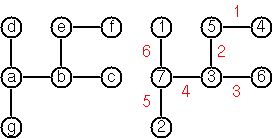
\includegraphics[scale=.2]{graphics/P92_1.png}  
% \end{figure}

Several years ago I met a mathematician who was intrigued by a problem
for which he didn't know a solution. His name was Von Koch, and I
don't know whether the problem has been solved since.

Anyway the puzzle goes like this: Given a tree with N nodes (and hence
N-1 edges). Find a way to enumerate the nodes from 1 to N and,
accordingly, the edges from 1 to N-1 in such a way, that for each edge
K the difference of its node numbers equals to
K. The conjecture is that this is always possible. 


% \begin{figure}[H]
%   \centering
% 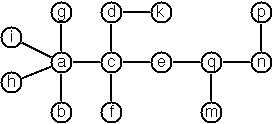
\includegraphics[scale=.6]{graphics/P92_2.png}
% \end{figure}


For small trees the problem is easy to solve by hand. However, for
larger trees, and 14 is already very large, it is extremely difficult
to find a solution. And remember, we don't know for sure whether there
is always a solution!

Write a predicate that calculates a numbering scheme for a given tree.
What is the solution for the larger tree pictured above?

\begin{wideverbatim}

We represent the tree as nested lists in the form

# edge:  number
# node:  (number . name)
# tree:  (edge node [tree ..])

For example, the representation of the first example's solution is

   (7 (7 . a)
      (4 (3 . b)
         (3 (6 . c))
         (2 (5 . e)
            (1 (4 . f)) ) )
      (6 (1 . d))
      (5 (2 . g)) )

The function 'kochConjecture' iterates a tree skeleton like

(0 (0 . a)
   (0 (0 . b)
      (0 (0 . c))
      (0 (0 . e)
         (0 (0 . f)) ) )
   (0 (0 . d))
   (0 (0 . g)) ) )

to obtain solutions like the one above.

\end{wideverbatim}

\begin{wideverbatim}


(de kochConjecture (Tree)
   (let
      (Cnt                             # Calculate number of nodes
         (recur (Tree)
            (if Tree
               (inc (sum recurse (cddr Tree)))
               0 ) )
         Edges (range 1 (dec Cnt))     # List of edge numbers
         Nodes (range 1 Cnt)           # List of node numbers
         L Nodes )
      (set Tree Cnt)                   # Set top edge (just for symmetry)
      (unless
         (recur (L)                    # Generate node number permutations
            (if (cdr L)
               (do (length L)
                  (NIL (recurse (cdr L)))
                  (rot L) )
               (use Nodes                 # Try next node number permutation
                  (recur (Tree)
                     (set (cadr Tree) (pop 'Nodes))
                     (mapc recurse (cddr Tree)) ) )
               (use Edges                 # Try to fit edges
                  (recur (Tree)
                     (let N (caadr Tree)  # Node number
                        (find
                           '((X)
                              (let E (abs (- N (caadr X)))  # Calculate edge
                                 (or
                                    (not (member E Edges))
                                    (prog
                                       (del E 'Edges)
                                       (set X E)
                                       (recurse X) ) ) ) )
                           (cddr Tree) ) ) ) ) ) )
         Tree ) ) )

\end{wideverbatim}

\begin{wideverbatim}


Test run (using 'pretty' to pretty-print the result):

(pretty
   (kochConjecture
      (0 (0 . a)
         (0 (0 . b))
         (0 (0 . c)
            (0 (0 . d)
               (0 (0 . k)) )
            (0 (0 . e)
               (0 (0 . q)
                  (0 (0 . m))
                  (0 (0 . n)
                     (0 (0 . p)) ) ) )
            (0 (0 . f)) )
         (0 (0 . g))
         (0 (0 . h))
         (0 (0 . i)) ) ) )

This returns as the first solution

(14
   (1 . a)
   (1 (2 . b))
   (13
      (14 . c)
      (11 (3 . d) (9 (12 . k)))
      (3
         (11 . e)
         (6
            (5 . q)
            (2 (7 . m))
            (5 (10 . n) (4 (6 . p))) ) )
      (10 (4 . f)) )
   (7 (8 . g))
   (8 (9 . h))
   (12 (13 . i)) )

\end{wideverbatim}

\pagebreak{}
\subsection*{{P93} (***) An arithmetic puzzle}
\label{sec:99-problems-P93}

Given a list of integer numbers, find a correct way of inserting
arithmetic signs (operators) such that the result is a correct equation.
Example: With the list of numbers (2 3 5 7 11) we can form the equations
2-3+5+7 = 11 or 2 = (3*5+7)/11 (and ten others!).

\begin{wideverbatim}

(de infix (E)
   (if (atom E)
      E
      (list
         (infix (cadr E))
         (car E)
         (infix (caddr E)) ) ) )

(de expressions (X)
   (if (cdr X)
      (mapcan
         '((I)
            (mapcan
               '((A)
                  (mapcan
                     '((B)
                        (mapcar
                           '((Op) (list Op A B))
                           '(+ - * /) ) )
                     (expressions (tail (- I) X)) ) )
               (expressions (head I X)) ) )
         (range 1 (dec (length X))) )
      (list (car X)) ) )

\end{wideverbatim}

\begin{wideverbatim}


(de equations (Lst)
   (use /
      (redef / (A B)
         (and (n0 B) (=0 (% A B)) (/ A B)) )
      (for (I 1  (> (length Lst) I)  (inc I))
         (for A (expressions (head I Lst))
            (for B (expressions (tail (- I) Lst))
               (let? N (eval A)
                  (when (= N (eval B))
                     (println (infix A) '= (infix B)) ) ) ) ) ) ) )

Test:

: (equations (2 3 5 7 11))
2 = (3 - (5 + (7 - 11)))
2 = (3 - ((5 + 7) - 11))
2 = ((3 - 5) - (7 - 11))
2 = ((3 - (5 + 7)) + 11)
2 = (((3 - 5) - 7) + 11)
2 = (((3 * 5) + 7) / 11)
(2 * (3 - 5)) = (7 - 11)
(2 - (3 - (5 + 7))) = 11
(2 - ((3 - 5) - 7)) = 11
((2 - 3) + (5 + 7)) = 11
((2 - (3 - 5)) + 7) = 11
(((2 - 3) + 5) + 7) = 11
-> NIL

\end{wideverbatim}

\pagebreak{}
\subsection*{{P95} (**) English number words}
\label{sec:99-problems-P95}

On financial documents, like cheques, numbers must sometimes be written
in full words. Example: 175 must be written as ``one hundred
seventy-five''. Write a function `fullWords' to return (non-negative)
integer numbers in full words.

\begin{wideverbatim}

(de fullWords (N)
   (cond
      ((=0 N) "zero")
      ((> 14 N)
         (get
         '("one" "two" "three" "four" "five" "six" "seven" "eight"
         "nine" "ten" "eleven" "twelve" "thirteen")
            N ) )
      ((= 15 N) "fifteen")
      ((= 18 N) "eighteen")
      ((> 20 N) (pack (fullWords (% N 10)) "teen"))
      ((> 100 N)
         (pack
            (get
               '("twen" "thir" "for" "fif" "six" "seven" "eigh" "nine")
               (dec (/ N 10)) )
            "ty"
            (unless (=0 (% N 10))
               (pack "-" (fullWords (% N 10))) ) ) )
      ((rank N '((100 . "hundred") (1000 . "thousand") (1000000 . "million")))
         (pack (fullWords (/ N (car @))) " " (cdr @) " " (fullWords (% N (car @)))) ) ) )

\end{wideverbatim}

\pagebreak{}
\subsection*{{P96} (**) Syntax checker}
\label{sec:99-problems-P96}

% \begin{figure}[H]
%   \centering
%   \includegraphics[scale=.6]{graphics/P96_1.png}
% \end{figure}

In a certain programming language (Ada) identifiers are defined by the
syntax diagram (railroad chart) opposite. Transform the syntax diagram
into a system of syntax gndiagrams which do not contain loops; i.e.
which are purely recursive. Using these modified diagrams, write a
function `identifier' that can check whether or not a given string is
a legal identifier.

\begin{wideverbatim}

(de identifier (Str)
   (and
      (>= "z" (lowc (car (setq Str (chop Str)))) "a")
      (not
         (find
            '((C)
               (nor
                  (= "_" C)
                  (>= "9" C "0")
                  (>= "z" (lowc C) "a") ) )
            (cdr Str) ) ) ) )

\end{wideverbatim}


\pagebreak{}
\subsection*{{P97} (**) Sudoku}
\label{sec:99-problems-P97}

Sudoku puzzles go like this:

\begin{wideverbatim}
Problem statement                 Solution

 .  .  4 | 8  .  . | .  1  7      9  3  4 | 8  2  5 | 6  1  7
         |         |                      |         |
 6  7  . | 9  .  . | .  .  .      6  7  2 | 9  1  4 | 8  5  3
         |         |                      |         |
 5  .  8 | .  3  . | .  .  4      5  1  8 | 6  3  7 | 9  2  4
 --------+---------+--------      --------+---------+--------
 3  .  . | 7  4  . | 1  .  .      3  2  5 | 7  4  8 | 1  6  9
         |         |                      |         |
 .  6  9 | .  .  . | 7  8  .      4  6  9 | 1  5  3 | 7  8  2
         |         |                      |         |
 .  .  1 | .  6  9 | .  .  5      7  8  1 | 2  6  9 | 4  3  5
 --------+---------+--------      --------+---------+--------
 1  .  . | .  8  . | 3  .  6      1  9  7 | 5  8  2 | 3  4  6
         |         |                      |         |
 .  .  . | .  .  6 | .  9  1      8  5  3 | 4  7  6 | 2  9  1
         |         |                      |         |
 2  4  . | .  .  1 | 5  .  .      2  4  6 | 3  9  1 | 5  7  8
\end{wideverbatim}

Every spot in the puzzle belongs to a (horizontal) row and a (vertical)
column, as well as to one single 3x3 square (which we call ``square''
for short). At the beginning, some of the spots carry a single-digit
number between 1 and 9. The problem is to fill the missing spots with
digits in such a way that every number between 1 and 9 appears exactly
once in each row, in each column, and in each square.

\begin{wideverbatim}

(load "@lib/simul.l")

### Fields/Board ###
# val lst

(setq
   *Board (grid 9 9)
   *Fields (apply append *Board) )

# Init values to zero (empty)
(for L *Board
   (for This L
      (=: val 0) ) )

# Build lookup lists
(for (X . L) *Board
   (for (Y . This) L
      (=: lst
         (make
            (let A (* 3 (/ (dec X) 3))
               (do 3
                  (inc 'A)
                  (let B (* 3 (/ (dec Y) 3))
                     (do 3
                        (inc 'B)
                        (unless (and (= A X) (= B Y))
                           (link
                              (prop (get *Board A B) 'val) ) ) ) ) ) )
            (for Dir '(`west `east `south `north)
               (for (This (Dir This)  This  (Dir This))
                  (unless (memq (:: val) (made))
                     (link (:: val)) ) ) ) ) ) ) )

# Cut connections (for display only)
(for (X . L) *Board
   (for (Y . This) L
      (when (member X (3 6))
         (con (car (val This))) )
      (when (member Y (4 7))
         (set (cdr (val This))) ) ) )


\end{wideverbatim}

\begin{wideverbatim}

# Display board
(de display ()
   (disp *Board 0
      '((This)
         (if (=0 (: val))
            "   "
            (pack " " (: val) " ") ) ) ) )

# Initialize board
(de main (Lst)
   (for (Y . L) Lst
      (for (X . N) L
         (put *Board X (- 10 Y) 'val N) ) )
   (display) )

# Find solution
(de go ()
   (unless
      (recur (*Fields)
         (with (car *Fields)
            (if (=0 (: val))
               (loop
                  (NIL
                     (or
                        (assoc (inc (:: val)) (: lst))
                        (recurse (cdr *Fields)) ) )
                  (T (= 9 (: val)) (=: val 0)) )
               (recurse (cdr *Fields)) ) ) )
      (display) ) )


\end{wideverbatim}

\begin{wideverbatim}

### Usage ###
: (main
   (quote
      (0 0 4 8 0 0 0 1 7)
      (6 7 0 9 0 0 0 0 0)
      (5 0 8 0 3 0 0 0 4)
      (3 0 0 7 4 0 1 0 0)
      (0 6 9 0 0 0 7 8 0)
      (0 0 1 0 6 9 0 0 5)
      (1 0 0 0 8 0 3 0 6)
      (0 0 0 0 0 6 0 9 1)
      (2 4 0 0 0 1 5 0 0) ) )
   +---+---+---+---+---+---+---+---+---+
 9 |         4 | 8         |     1   7 |
   +   +   +   +   +   +   +   +   +   +
 8 | 6   7     | 9         |           |
   +   +   +   +   +   +   +   +   +   +
 7 | 5       8 |     3     |         4 |
   +---+---+---+---+---+---+---+---+---+
 6 | 3         | 7   4     | 1         |
   +   +   +   +   +   +   +   +   +   +
 5 |     6   9 |           | 7   8     |
   +   +   +   +   +   +   +   +   +   +
 4 |         1 |     6   9 |         5 |
   +---+---+---+---+---+---+---+---+---+
 3 | 1         |     8     | 3       6 |
   +   +   +   +   +   +   +   +   +   +
 2 |           |         6 |     9   1 |
   +   +   +   +   +   +   +   +   +   +
 1 | 2   4     |         1 | 5         |
   +---+---+---+---+---+---+---+---+---+
     a   b   c   d   e   f   g   h   i
-> NIL


\end{wideverbatim}

\begin{wideverbatim}


: (go)
   +---+---+---+---+---+---+---+---+---+
 9 | 9   3   4 | 8   2   5 | 6   1   7 |
   +   +   +   +   +   +   +   +   +   +
 8 | 6   7   2 | 9   1   4 | 8   5   3 |
   +   +   +   +   +   +   +   +   +   +
 7 | 5   1   8 | 6   3   7 | 9   2   4 |
   +---+---+---+---+---+---+---+---+---+
 6 | 3   2   5 | 7   4   8 | 1   6   9 |
   +   +   +   +   +   +   +   +   +   +
 5 | 4   6   9 | 1   5   3 | 7   8   2 |
   +   +   +   +   +   +   +   +   +   +
 4 | 7   8   1 | 2   6   9 | 4   3   5 |
   +---+---+---+---+---+---+---+---+---+
 3 | 1   9   7 | 5   8   2 | 3   4   6 |
   +   +   +   +   +   +   +   +   +   +
 2 | 8   5   3 | 4   7   6 | 2   9   1 |
   +   +   +   +   +   +   +   +   +   +
 1 | 2   4   6 | 3   9   1 | 5   7   8 |
   +---+---+---+---+---+---+---+---+---+
     a   b   c   d   e   f   g   h   i
-> NIL

\end{wideverbatim}

\pagebreak{}
\subsection*{{P98} (***) Nonograms}
\label{sec:99-problems-P98}

Around 1994, a certain kind of puzzles was very popular in England. The
``Sunday Telegraph'' newspaper wrote: ``Nonograms are puzzles from Japan
and are currently published each week only in The Sunday Telegraph.
Simply use your logic and skill to complete the grid and reveal a
picture or diagram.'' As a PicoLisp programmer, you are in a better
situation: you can have your computer do the work! Just write a little
program ;-).

 The puzzle goes like this: Essentially, each row and
column of a rectangular bitmap is annotated with the respective lengths
of its distinct strings of occupied cells. The person who solves the
puzzle must complete the bitmap given only these lengths.

\begin{wideverbatim}
   Problem statement:          Solution:

   |_|_|_|_|_|_|_|_| 3         |_|X|X|X|_|_|_|_| 3
   |_|_|_|_|_|_|_|_| 2 1       |X|X|_|X|_|_|_|_| 2 1
   |_|_|_|_|_|_|_|_| 3 2       |_|X|X|X|_|_|X|X| 3 2
   |_|_|_|_|_|_|_|_| 2 2       |_|_|X|X|_|_|X|X| 2 2
   |_|_|_|_|_|_|_|_| 6         |_|_|X|X|X|X|X|X| 6
   |_|_|_|_|_|_|_|_| 1 5       |X|_|X|X|X|X|X|_| 1 5
   |_|_|_|_|_|_|_|_| 6         |X|X|X|X|X|X|_|_| 6
   |_|_|_|_|_|_|_|_| 1         |_|_|_|_|X|_|_|_| 1
   |_|_|_|_|_|_|_|_| 2         |_|_|_|X|X|_|_|_| 2
   1 3 1 7 5 3 4 3             1 3 1 7 5 3 4 3
   2 1 5 1                     2 1 5 1
\end{wideverbatim}             

For the example above, the problem can be stated as the two lists ((3)
(2 1) (3 2) (2 2) (6) (1 5) (6) (1) (2)) and ((1 2) (3 1) (1 5) (7 1)
(5) (3) (4) (3)) which give the ``solid'' lengths of the rows and
columns, top-to-bottom and left-to-right, respectively. Published
puzzles are larger than this example, e.g. 25 x 20, and apparently
always have unique solutions.


\begin{wideverbatim}

(de nonogram (LstX LstY)
   (let Lim (** 2 (length LstY))
      (_nonogX LstX) ) )

(de _nonogX (LstX Res)
   (if LstX
      (_nonogY LstX Res)
      (when
         (= LstY
            (make
               (for (I Lim (gt0 (setq I (>> 1 I))))
                  (link
                     (flip
                        (make
                           (let C NIL
                              (for N Res
                                 (if2 (bit? I N) C
                                    (inc 'C)
                                    (one C)
                                    (prog (link C) (off C)) ) )
                              (and C (link @)) ) ) ) ) ) ) )
         (for N (flip Res)
            (for (I Lim (gt0 (setq I (>> 1 I))))
               (prin "|" (if (bit? I N) "X" "_")) )
            (prinl "|") ) ) ) )


\end{wideverbatim}

\begin{wideverbatim}


(de _nonogY (LstX Res)
   (let (Lst (mapcar '((N) (cons 1 (** 2 N))) (car LstX))  P Lst)
      (recur (P)
         (ifn P
            (let N 0
               (for X Lst
                  (setq N
                     (+
                        (* 2 N (car X) (cdr X))
                        (* (car X) (dec (cdr X))) ) ) )
               (when (> Lim N)
                  (_nonogX (cdr LstX) (cons N Res))
                  T ) )
            (prog1 (recurse (cdr P))
               (while
                  (prog
                     (set (car P) (* 2 (caar P)))
                     (recurse (cdr P)) ) )
               (set (car P) 1) ) ) ) ) )

: (nonogram
   '((3) (2 1) (3 2) (2 2) (6) (1 5) (6) (1) (2))
   '((1 2) (3 1) (1 5) (7 1) (5) (3) (4) (3)) )
|_|X|X|X|_|_|_|_|
|X|X|_|X|_|_|_|_|
|_|X|X|X|_|_|X|X|
|_|_|X|X|_|_|X|X|
|_|_|X|X|X|X|X|X|
|X|_|X|X|X|X|X|_|
|X|X|X|X|X|X|_|_|
|_|_|_|_|X|_|_|_|
|_|_|_|X|X|_|_|_|
-> T

\end{wideverbatim}

\pagebreak{}
\subsection*{{P99} (***) Crossword puzzle}
\label{sec:99-problems-P99}

Given an empty (or almost empty) framework of a crossword puzzle and a
set of words. The problem is to place the words into the framework.

% \begin{figure}[H]
%   \centering
%    \includegraphics[scale=.6]{graphics/P99_1.png}  
% \end{figure}

The particular crossword puzzle is specified in a text file which
first lists the words (one word per line) in an arbitrary order. Then,
after an empty line, the crossword framework is defined. In this
framework specification, an empty character location is represented by
a dot (.). In order to make the solution easier, character locations
can also contain predefined character values. The puzzle opposite is
defined in the file \href{!wiki?99p99a}{p99a.dat}, other examples are
\href{!wiki?99p99b}{p99b.dat} and \href{!wiki?99p99d}{p99d.dat}. There
is also an example of a puzzle (\href{!wiki?99p99c}{p99c.dat}) which
does not have a solution.

\emph{Words} are strings (character lists) of at least two characters.
A horizontal or vertical sequence of character places in the crossword
puzzle framework is called a \emph{site}.

Our problem is to find a compatible way of placing words onto sites.

\begin{wideverbatim}

(load "@lib/simul.l")

(de crossword (File)
   (use (Words Data Grid Slots Org)
      (in File
         (setq
            Words (flip (by length sort (make (while (line) (link (trim @))))))
            Data (flip (make (while (line) (link (trim @)))))   # Read data
            Len (apply max (mapcar length Data))
            Grid (grid Len (length Data)) ) )            # Create grid
      (for Col Grid  # Set initial data
         (use Data
            (for This Col
               (let C (pop Data)
                  (=: char (unless (sp? C) C)) )
               (pop 'Data) ) ) )
      (setq Slots
         (mapcar
            '((L) (cons (length (car L)) L))
            (by length group
               (make
                  (for Col Grid  # Init slots
                     (for This Col
                        (when (: char)
                           (and  # Check horizontal slot
                              (not (; (west This) char))
                              (; (east This) char)
                              (; (east (east This)) char)
                              (link
                                 (make
                                    (for (This This (: char) (east This))
                                       (link This) ) ) ) )
                           (and  # Check vertical slot
                              (not (; (north This) char))
                              (; (south This) char)
                              (; (south (south This)) char)
                              (link
                                 (make
                                    (for (This This (: char) (south This))
                                       (link This) ) ) ) ) ) ) ) ) ) ) )

\end{wideverbatim}

\begin{wideverbatim}


      (recur (Words)
         (if Words
            (for Slot (cdr (assoc (length (car Words)) Slots))
               (unless
                  (find
                     '((This C) (nor (= C (: char)) (= "." (: char))))
                     Slot
                     (car Words) )
                  (let Org (mapcar get Slot '(char .))
                     (mapc put Slot '(char .) (car Words))
                     (recurse (cdr Words))
                     (mapc put Slot '(char .) Org) ) ) )
            (disp Grid T  # Found a solution: Display it
               '((This)
                  (if (: char)
                     (pack " " @ " ")
                     "###" ) ) ) ) ) ) )

: (crossword "p99a.dat")

   +---+---+---+---+---+---+---+---+---+
 6 | P | R | O | L | O | G |###|###| E |
   +---+---+---+---+---+---+---+---+---+
 5 | E |###| N |###|###| N |###|###| M |
   +---+---+---+---+---+---+---+---+---+
 4 | R |###| L | I | N | U | X |###| A |
   +---+---+---+---+---+---+---+---+---+
 3 | L |###| I |###| F |###| M | A | C |
   +---+---+---+---+---+---+---+---+---+
 2 |###|###| N |###| S | Q | L |###| S |
   +---+---+---+---+---+---+---+---+---+
 1 |###| W | E | B |###|###|###|###|###|
   +---+---+---+---+---+---+---+---+---+
     a   b   c   d   e   f   g   h   i

\end{wideverbatim}


\pagebreak{}
 \textbf{Hints:}

 (1) The problem is not easy. You will need some time to thoroughly
 understand it. So, don't give up too early! And remember that the
 objective is a clean solution, not just a quick-and-dirty hack!

 (2) Reading the data file is a tricky problem (in Prolog?).

 (3) For efficiency reasons it is important, at least for larger
 puzzles, to sort the words and the sites in a particular order. For
 this part of the problem, the solution of P28 may be very helpful.

